\label{sec:background}
\subsection{Literature on the value of political connections}
\citet{pena2018privatization} use data from 1995-2003 for 25 European countries to conclude that the perceived level of corruption increases with privatizations. However, the impact increase with the economic relevance of the privatization. This could perhaps be a factor in explaining the consistent low level of perceived corruption in Denmark regardless of the evidence of a wide transfer of rent from municipalities to mostly unprofitable firms owned by family members of local politicians \citep{amore2013value}.

In Spain, a country in which perceived corruption is significantly higher, \citet{albalate2017weakening} find clear evidence of favoritism of a certain firm in municipalities where the conservative party is in power. However, this form of rent seeking was successfully reduced by two reforms in 2007, that is, by increasing transparency and use of external referees in bidding processes while banning donations to political parties from firms with public sector contracts. Though these reforms had a clear positive effect Spain still ranked as having one of the highest risks of bribery of any developed country in the TRACE index constructed by RAND Corporation \citep{stanley2014business}. In the the same index Denmark rank as the worst of the Nordic countries while Japan is estimated to have the \nth{8} lowest business bribery risk score in the World, wherefore it is doubtable how big of a potential there is for similar regulatory reforms in Japan.

\subsection{Political institutions and norms in Japan}
Taking a closer look at Japan in the TRACE matrix developed by the RAND Corporation \citep{stanley2014business} the overall risk of business bribery is decomposed into scores in 4 main areas as seen in figure \ref{tab:trace}. Though the expectation of a bribe transaction in an interaction between businesses and the government is low, the high amount of interactions and regulations are the only real contributors to increasing the overall risk of bribery in Japan, having impressively low risk scores in every other category. The amount and quality of anti-bribery laws are regarded much higher than for Denmark and Spain even more so is Japan regarded the best performing country in the World when it comes to transparency of various government functions while having a very trustworthy and/or oversighted civil service workforce. Lastly, the quality and independence of the media is regarded slightly higher than for Denmark and Spain while all three countries have a relatively well-educated and economically stable population likely to object corruption.
\begin{table}[H]
  \centering
  \caption{TRACE Matrix of business bribery risk}
  \footnotesize
    \begin{tabular}{lccc}
\toprule
Domain / subdomain  & Japan & Denmark & Spain \\
\midrule
TRACE Rank                                &  8 & 21 & 36 \\
Total risk of business bribery            & 26 & 32 & 41 \\
\midrule
1.0 Business Interactions with Government & 33 & 24 & 47 \\
\ 1.1 Contact with Government             & 36 & 13 & 39 \\
\ 1.2 Expectation of Paying Bribes        & 14 & 14 & 39 \\
\ 1.3 Regulatory Burden                   & 51 & 52 & 57 \\
\midrule
2.0 Anti-Bribery Laws and Enforcement     & 17 & 52 & 31 \\
\ 2.1 De Jure Anti-Bribery Laws           & 24 & 56 & 42 \\
\ 2.2 De Facto Anti-Bribery Enforcement   & 12 & 48 & 22 \\
\midrule
3.0 Government and Civil Service Transparency             &  6 & 39 & 35 \\
\ 3.1 Transparency of Government Regulatory Functions     &  1 & 36 & 31 \\
\ 3.2 Transparency and Health of the Civil Service Sector & 23 & 47 & 45 \\
\midrule
4.0 Capacity for Civil Society Oversight  & 10 & 20 & 14 \\
\ 4.1 Quality and Freedom of Media        & 14 & 27 & 17 \\
\ 4.2 Human Capital and Social Development&  8 &  9 & 12 \\
\bottomrule
\end{tabular}
%
% \usepackage{float}
%
% \begin{table}[H]
%   \centering
%   \caption{Example of table}
%   \footnotesize
%     \begin{tabular}{lrrrr}
\toprule
Year, month   & Cities  & Towns & Villages  & Total \\
\midrule

\bottomrule
\end{tabular}
%
% \usepackage{float}
%
% \begin{table}[H]
%   \centering
%   \caption{Example of table}
%   \footnotesize
%     \begin{tabular}{lrrrr}
\toprule
Year, month   & Cities  & Towns & Villages  & Total \\
\midrule

\bottomrule
\end{tabular}
%
% \usepackage{float}
%
% \begin{table}[H]
%   \centering
%   \caption{Example of table}
%   \footnotesize
%     \input{04_tables/example}
%   \label{tab:ex}
% \end{table}

%   \label{tab:ex}
% \end{table}

%   \label{tab_example}
% \end{table}

    \sourcec{RAND Corporation \citep{stanley2014business}.}
  \label{tab:trace}
\end{table}\noindent
The higher risk scores for Denmark and Spain, especially in terms of anti-bribery laws and enforcement as well as the transparency of government and civil service, are likely to lay the foundation for the significant values of political connections found in studies for both countries \citep{amore2013value,albalate2017weakening}. The TRACE index suggests a lower risk of business bribery in Japan and can raise the question whether it is at all feasible to consistently extract rent from political connections.

Despite all the parameters that suggest a low risk of bribery \citep{stanley2014business} figure \ref{tab:CPI} suggest that the perceived level of corruption of the public in Japan is considerably and persistently higher than the countries at the top like Denmark which consistently have been taking one of the very-top spots of both Transparency International's Corruption Perceptions Index (CPI) and The World Bank's Worldwide Governance Indicators (WGI) \citep{rohwer2009measuring} since both was initiated in the mid 90s. The validity of these indexes have often been criticised for only being able to measure perceived corruption. However homogeneity and comparability is ensured by surveying business people were the finding is that there are minimal differences in perception between nationals and foreigners \citep{galtung2006measuring}. While the indexes have little external validation for the opinions of the population of a whole, they clearly show that business people to a larger degree experience openings for political favoritism and rent seeking in Japan than in several other countries. For all that, Japan is still perceived as the least corrupt country in Asia besides from the city-states of Singapore and Hong Kong.
\begin{table}[H]
  \centering
    \footnotesize
  \caption{Corruption Perceptions Index (CPI) 2017}
    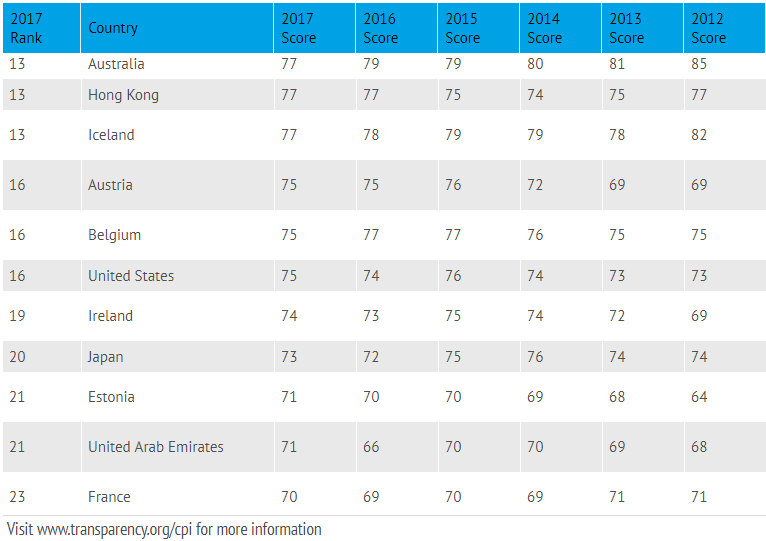
\includegraphics[width= \textwidth]{04_tables/CPI}
  \label{tab:CPI}
  \sourcel{\href{https://www.transparency.org/research/cpi}{Transparency International}. A score of $0$ is highly corrupt and $100$ is very clean.}
\end{table}\noindent
Analyzing 42 countries \citet{faccio2006politically} finds evidence in 35 countries of national politicians at the same time being shareholders or top managers in publicly traded firms. Japan is found to have the most connected politicians together with Malaysia, the UK, Germany and France. She also identifies 28 cases of businessmen entering national politics in Japan, bested only by the number of cases in the UK. However, she finds that rent transfer and tax advantages for connected firms is more evident in high-corruption countries while insignificant for Japan.

\subsection{Merging of municipalities}
Municipal autonomy was implemented back in 1889 with the merging of around 70,000 cities, towns and villages into about 15,000 municipalities. After World Ward II The Law for Promoting Municipal Mergers lead to the about 10,000 municipalities in 1953 being merged into just under 3,500 municipalities by 1961. A number that was quite stable until a \nth{3} wave of mergers known as the "Great Heisei Consolidation" where series of incentives including financial support for mergers was initiated April 1, 1999, and terminated by the end of March, 2006 \citep{michihiro2007local} with the clear effects shows in table \ref{tab:municipalities}\footnote{Since the \href{http://nippon.zaidan.info/seikabutsu/1999/00168/mokuji.htm}{The Local Autonomy law (1999 version, in English)} in 1947 there has been no difference in the political autonomy of cities, towns and villages respectively, but the terms are still used as an indication of size and degree of urban characteristics though it is not consistent.}. In this 7 year period the number of municipalities was reduced by 44\%.\footnote{\href{www.soumu.go.jp/gapei/gapei2.html}{The Ministry of Internal Affairs and Communications' overview of the number of municipalities over time (in Japanese)}}
\begin{table}[H]
  \centering
  \caption{Total number of municipalities by year}
  \footnotesize
    \begin{tabular}{lrrrr}
\toprule
Month, year & Cities& Towns & Villages& Total \\ Municipalities \\
\midrule
April 1975  & 643   & 1,974 & 640     & 3,257 \\
April 1999  & 671   & 1,990 & 568     & 3,229 \\
April 2002  & 675   & 1,981 & 562     & 3,218 \\
May 2004    & 695   & 1,872 & 533     & 3,100 \\
April 2005  & 739   & 1,317 & 339     & 2,395 \\
March 2006  & 777   &   846 & 198     & 1,821 \\
April 2010  & 786   &   757 & 184     & 1,727 \\
April 2014  & 790   &   745 & 183     & 1,718 \\
\bottomrule
\end{tabular}
%
% \usepackage{float}
%
% \begin{table}[H]
%   \centering
%   \caption{Example of table}
%   \footnotesize
%     \input{04_tables/elasticities}
%    \sourcec{}
%   \label{tab:elasticities}
% \end{table}

   \sourcec{Ministry of Internal Affairs and Communications.}
  \label{tab:municipalities}
\end{table}\noindent
The motivation for encouraging mergers was to decentralize government, utilize economies of scale, and handle challenges arising from demographics and local as well as national fiscal struggle \citet{yokomichi2007development}. While the political power per elected politician increases by merging of municipalities the electoral power decreases correspondingly and in the rural municipalities that had merged the level of public services has been perceived to have declined more compared to non-merged rural municipalities \citep{yamada2018majority}.

\subsection{Firm accounts and managers}
Statistics Bureau conduct the Economic Census\footnote{\href{http://www.stat.go.jp/english/data/e-census.html}{Statistics Bureau, Economic Census.}} in which they cover all firms in Japan in each of two surveys. The Economic Census For Business Activity include sales, expenses, assets, current stock, location, type, startup date and more. In the Economic Census For Business Frame all paid directors, managers, employees, and unpaid family workers are identified. It is also identified whether a firm is single-unit, a head office or a branch office as well as the industrial classifications of main and other business activities.

By late 2015 both Corporate Numbers and Individual Numbers were fully implemented, allowing for better identification of individuals across different registers.\footnote{\href{http://www.japaneselawtranslation.go.jp/law/detail/?id=2755&vm=04&re=02}{Act on the Use of Numbers to Identify a Specific Individual in Administrative Procedures.}}

\subsection{Electoral data and family trees}
Access to electoral data with party affiliation and ID numbers as well as information on family relations and spouses are necessary to build family trees and establish family-connections to firms. This is what fundamentally enrichens the analysis compared to being limited to a politician herself being directly involved in a firm.
